\chapter{Contexte des Réseaux sociaux Centralisés et décentralisés}
\section{Introduction}
\textit{QU'EST CE QU'UN RÉSEAU SOCIAL ?}\newline
Le terme "réseau social" provient de John Arundel Barnes en 1954.
Les réseaux sociaux existaient bien avant Internet. En effet, un réseau social n'est rien d'autre qu'un groupe de personnes ou d'organisations reliées entre elles entretiennent.
Un utilitaire social comme Facebook, GooglePlus ou autres aident les gens à communiquer de manière plus efficace avec les amis, la famille et les collègues. 
\subparagraph{}
Aujourd'hui le réseau social c'est une application internet dédiée à la communication avec ses connaissances, à la rencontre de nouvelles personnes, à la construction de son réseau professionnel, à la partage des données ou le sauvegarde des centres d'intérêt (des multimédias sur internet ou PC).
\subparagraph{}
Le principe de base est le même pour tous les réseaux sociaux :
Création d'un profile, 
Inviter des amis,
Accepter des contacts, 
Partager un contenu,
Discuter, ect…
Le plus important dans ce type de réseaux est de permettre à l'internaute d'augmenter ça réputation virtuelle.
\subparagraph{}
Les utilitaires sociaux Facebook, mySpace, LinkedIn, OrKut, GooglePlus, ect… gagnent chaque jour des millions d'utilisateurs, mais on commence à apercevoir quand même des utilisateurs qui désactive leurs comptes facebook ou autres. D'après \textit{l'article de BEGEEK} \footnote{http://www.begeek.fr/facebook-chute-daudience-et-une-perte-de-plusieurs-millions-dutilisateurs-91030 publié le 29 avril 2013 à 19h04}sur le chute de facebook :
Selon "SocialBakers", ces six derniers mois le réseau de Mark Zuckerberg aurait perdu neuf millions d’abonnés sur le sol américain.
\begin{wrapfigure}[12]{r}{6.5cm}
\vspace{-5mm}
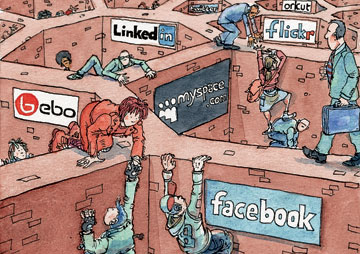
\includegraphics[width=7cm]{walled_garden.jpg}
\textbf{\caption{Problem with today's social networks\protect\footnote{http://dig.csail.mit.edu/2008/Papers/MSNWS/  Reproduction de www.economist.com}}}
\end{wrapfigure}
\subparagraph{}
Ces sites présentes trois problèmes majeurs:
Premièrement, c'est que les informations dans un site ne peuvent pas être utiliser dans les autres sites.
Deuxièmement, ces sites ne permettent pas au utilisateurs de contrôler leurs données personnelles diffusés ce qui entraîne des problèmes de confidentialité potentiels. Finalement, les données contrôler par la firme possessive des données au commerçant et puis c'est dernier il les revende au gouvernement dont il dépend, pour éspionner, réutiliser, ect... 
\subparagraph{}
Ces problèmes peuvent être résolue en adoptant une approche décentralisée pour les réseaux sociaux, avec cette approche les utilisateurs n'ont pas à être limitée par un service social.
Cette approche peut fournir le même niveau, acquérir un nombre bel et bien important d'utilisateurs tout en leur accordant plus de contrôle vis à vis leurs informations personnelles et maintenir mieux leur gestion.
\subparagraph{}
Le réseau social distribuée est basé sur les téchnologies ouvertes : Linked Data, les ontologies du web sémantique, les systèmes d'identités unique WEBID et le access contrôle (web access contrôle).
Les URIs des identificateurs permettent au framework décentralisée d'être distribuée extensible, comme les utilisateurs, les applications, les données référent à leurs URIs\footnote{http://dig.csail.mit.edu/2008/Papers/MSNWS/}.
Le web actuelle est décentralisé mais il n'est pas distribué, en effet Il forme le cercle vicieux contournant autour les geant comme Google, Amazon, ect...
\begin{figure}
                \centering
                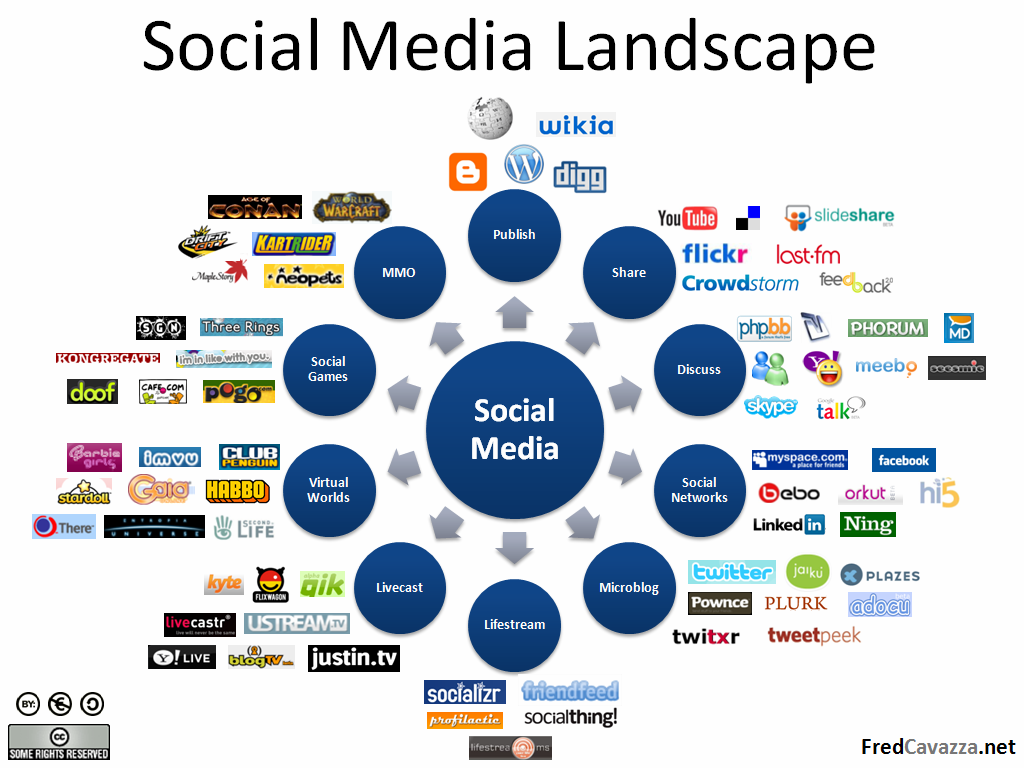
\includegraphics[width=\textwidth]{Social-Media-Landscape.png}
                \caption{Social Media}
                \label{fig:Social Media}      
\end{figure}

\newpage
\section{PARTIE 1 : Etude des réseaux sociaux existants}
\subsection{Les débuts décentralisés d‘internet} 
\paragraph{}
La modélisation d'un réseau social décentralisé qui élimine la dualité entre le fournisseur de service et l'utilisateur, le modèle client/serveur, remplacer par une situation ou chaque utilisateur à son propre serveur (chaque client est un serveur) c'est loin d'être une nouveauté absolu mais c'est plustôt c'est un retour aux origines d'internet.
\subparagraph{} 
En effet, depuis le début des "réseaux des réseaux" le principe de décentalisation a été à la base de transmission et de communication qui y circule.  Pourtant en 1990 l'introduction du web a conduit progressivement à un modèle client/serveur;  les services diffuser sur internet les plus répandus(les réseaux sociaux(Twitter), les services de stockage des données numérique(dropbox)…)
sont conçus à partir d'un modèle technique dans lesquels l'utilisateur final demande une donnée, information ou service à un puissant centre de serveurs qui stockent les informations et gèrent le trafic sur le réseau donc même sur internet si le trafic fonctionne avec le principe de distribution généralisée actuellement il est concentré autour de serveurs qui autorisent l'accès au contenu.
\subparagraph{}
Pourtant la conception d'un réseau distribué de façon que la communication/les échanges auront lieu entre des noeuds jouant un rôle symétrique dans le système. C'est une alternative possible qui est le plus à même d'assurer la durabilité du réseau internet.
\subsection{Motivation} 
\paragraph{}
Les services des réseaux sociaux existant sont centralisé la compagnie qui donne le service à tout le contrôle de l'information. Ce n'est pas facile à l'utilisateur de réutiliser ces propres données inclus son réseau social, le contenu multimédia dans d'autres plateforme. Jusqu'à maintenant il n'y a pas un mécanisme permettent de transporter les données d'un utilisateur d'une plateforme à une autre.
Essentiellement les gens s'ennui de crée un compte sur une nouvelle plateforme puis re-ajouter tous leurs amis en ligne, informations, ect… 
Et puis la présentation de leurs informations est souvent dépendante du design du service social qu'ils utilisent.
\subparagraph{}
De plus les utilisateurs doivent accepter les conditions générales d'utilisation de ces réseaux sociaux quand ils les utilisent, ainsi qu'ils peuvent accepter l'utilisation de leurs données. En outre, très souvent, les utilisateurs doivent explicitement "opt-out" de certaines applications si elles sont plus conscients de la confidentialité de leurs données. Cependant, avec un contrôle décentralisé, pas un seul service est le seul accès aux données et la capacité d'appliquer les décisions arbitraires.
\subparagraph{}
Les réseaux sociaux populaires comme Facebook, GooglePlus et autres donnent l'impression à leurs utilisateurs qu'ils ne contrôlent pas les données, par contre ce n'est pas le cas. Par exemple Facebook donne la possibilité aux utilisateurs de désactiver leurs compte, mais ce n'est pas possible d'écraser tous les données et les informations personnelles misent sur le serveur du site.
\newpage
\section{PARTIE 2 : A propos des réseaux sociaux décentralisés}
\subsection{Le décentralisé sur le Net }
\paragraph{}
Un nombre de projet actuellement relèvent le défi à créer le réseau social décentralisé qui puisse ériger à compétiteur crédible et fiable de Facebook.
  \begin{center}
------------------------------------------------------
\end{center}
\begin{itemize}
  \item Diaspora \footnote{https://diasporafoundation.org/about} : 
\subparagraph{}
Diaspora c'est le premier réseau social décentralisé qui a eu un très grand écho dans les médias histoire ou différentes ordinateurs indépendant dits "graines" sont amenés directement entre eux tout en abritant leurs propre profil.

- NoseRub \footnote{http://en.wikipedia.org/wiki/Noserub} : 
\subparagraph{}
C'est un protocole distribué sous licence MIT (Massachusetts Institute of Technology) 
il a été créé par Dirk Olbertz, permettant aux utilisateurs de réseau de garder les information de leur profile sur leur propre terminaux, et à leurs terminaux d'interagir et de se synchroniser automatiquement.
  \item TENT \footnote{https://tent.io/about}: 
\subparagraph{}
Tent est un protocole de communication distribués. Tent peut être utilisé comme un emplacement de stockage personnel des données, un seul signe sur le service, et / ou un réseau social distribué. N'importe qui peut héberger leur propre serveur de tent. En plus d'accueillir des tents, Tent.is donne quelques applications de base pour aider les utilisateurs à démarrer, une application d'administration du serveur et une application de micro-blogging.
\subparagraph{}
""Both the protocol / open source staff and Tent.is are built and maintained by the same team which is half American, half Canadian, ect...""
N'importe quelle personne peux crée un serveur Tent. Il n'est pas centralisé pour limiter les autorités des développeurs ou les utilisateurs.
\subparagraph{}
Les posts sont au coeur de tent protocole, Chaque morceau de données dans la tent, à partir d'un message d'état de configuration de l'application, est stockée dans un post.

Les Posts sont du JSON consiste de trois composants logic :
\begin{itemize}
  \item metadata 
 \item content 
 \item binary attachment
\end{itemize}

1) Tent vous permet de sauvegarder vos données dans une place dont vous avez le contrôle. 

2) Vous pouvez choisir un fournisseur d'hébergement ou lancer votre propre serveur.

3) Si vous souhaitez déplacer les hosts vous aurez vos données et relations.
\begin{itemize}
  \item tent utilise https et JSON pour transporter les posts entre les serveurs et les apps.
\item les entités sont les utilisateurs de tant il autorisent apps, établi des relations et lire/publier des posts les entités sont définie avec leur entité URL; https/http URL liée les métadata
\item chaque entité a 1 ou plusieurs serveur qui la représente.
\item posts sont les atomics unité de contenu dans tent chaque post est un JSON, ils ont des fichiers attacher.
\item APPS fourni des UI (user interface) pour tent.
\item tent c'est une machine readable JSON api les apps doivent être autorisée avec oauth2
\item relationShips : les entités établissent des relations lorsque il envoient des messages qui mentionnent d'autres entités. 

\end{itemize}
\subparagraph{}
Les fonctionnalités trouvées aussi sur les sites d'information communautaires comme \textit{hacker news} \footnote{http://thehackernews.com/} peuvent être reproduite avec tent, mais nécessairement architecturée d'une manière différente. les messages et les commentaires sont situé sur le serveur tent au lieu d'être regroupé sur un site unique ou base de donnée. 
\subparagraph{}
Les données sont stockées dans tent comme messages. Messages, comme les fichiers, sont tapés. Il ya un petit nombre de types de poste prévues par le protocole que les serveurs utilisent des tentes. Les développeurs sont libres de créer de nouveaux types de poste pour le contenu / stockage de données.

  \item En france Turbulences \footnote{http://ticmigrations.fr/fr/etat-de-lart/projets/116-turbulence} :
\subparagraph{}
 Propose une solution technologique open-source, utilisant pour une variété d'acteurs institutionnels et de secteur privé afin d'assembler et de lancer leur service de réseau social, intégré au services en ligne existant au travers de protocoles et de standards libres.

\textbf{On peut cité aussi }
\item Freenet \footnote{http://fr.wikipedia.org/wiki/Freenet} : C'est un réseau informatique anonyme et distribué construit sur l'Internet. Il vise à permettre une liberté d'expression et d'information totale fondée sur la sécurité de l'anonymat, et permet donc à chacun de lire comme de publier du contenu. Il offre la plupart des services actuels d'Internet (courriel, Web, etc.). 

\textit{C'est deux derniers réseaux ne sont pas des réseaux sociaux distribué mais ils font du distribué. }
\end{itemize}
\subsection{Réseautage social décentralisé en ligne}
\textit{Description d'un style d'architecture distribuée}\newline
\paragraph{}
Dans un cadre de réseau social distribué et ouvert, un utilisateur n'a pas besoin d'adhérer à un service particulier de réseautage social tels que Facebook ou MySpace. Au lieu de cela, l'utilisateur choisit un serveur qui il a confiance pour héberger ses propres données telles que son FOAF (Friend-Of-A-Friend) [ fichier, son journal d'activité et ses albums photos. Étant donné que nous nous référons à ces fichiers avec leurs URI, ils peuvent effectivement être stockés sur des serveurs différents\footnote{http://dig.csail.mit.edu/2008/Papers/MSNWS/}.

\subparagraph{}
En utilisant FOAF dans un cadre de mise en réseau social décentralisé, le WEBID d'un utilisateur peut être utilisé comme un point d'accès à ses données. Les autres utilisateurs qui veulent accéder au réseau de l'utilisateur sociaux (liste d'amis), son statut, ses photos, ou d'écrire sur son tableau de message personnel, seront versés à son dossier de FOAF et obtenir les URI correspondant. En stockant les données dans un serveur de confiance choisie par l'utilisateur, les utilisateurs ont plus de contrôle sur les données. 
\subparagraph{}
Il ya aussi une option pour créer des politiques de contrôle d'accès à grains fins beaucoup en utilisant des langages de la politique comme de l'air [Kagal et al. 2008] pour aider à limiter l'accès à ses données ou des applications. Contrairement à un site centralisé de réseautage social, les utilisateurs devront s'authentifier sur des serveurs différents quand ils veulent accéder aux données confidentielles de leurs amis. 
\subparagraph{}
Cela peut être fait en utilisant par exemple le protocole OpenID [Recordon et Fitzpatrick 2006] en permettant aux utilisateurs de créer des identités en ligne qui utilisent des protocoles existants comme URI, HTTP, SSL et Diffie-Hellma etc ou en utilisant FOAF des utilisateurs + certificats SSL . Un tel cadre décentralisé permet également une personnalisation plus importante des applications et des interfaces. Par exemple, les utilisateurs peuvent créer leur propre page d'accueil qui montre leur réseau, des activités et des photos en ligne sociaux.
\begin{figure}
        \centering
                \centering
                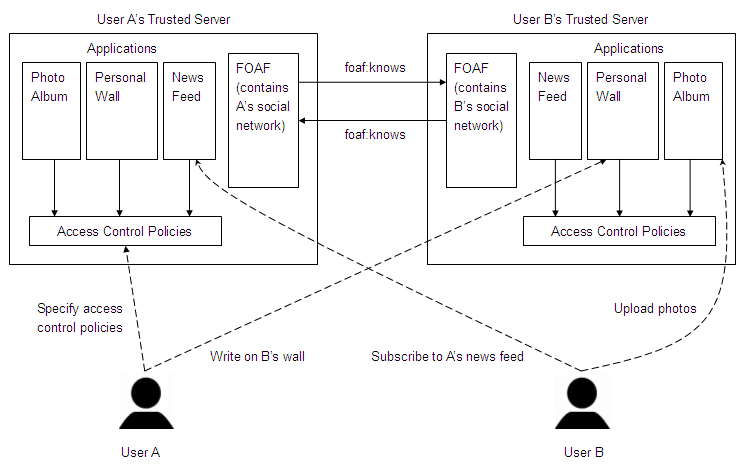
\includegraphics[width=\textwidth]{framework.png}
                \caption{A framework of decentralized online social networking}
                \label{fig:A framework of decentralized online social networking}
       
\end{figure}
\newpage
\section{Conclusion du chapitre 5}
\paragraph{}
\textit{Ces alternatives de réseaux sociaux décentralisé prendra-t-elle suffisamment pied pour constitué un véritable défi pour le géant Facebook ?}
\subparagraph{}
Le point d'interrogation principale concerne sans doute la réceptivité des utilisateurs à la possibilité de migrer non seulement sur une nouvelle plate-forme, mais aussi sur une application dans la prise en main, la facilité d'utilisation et les bénéfices sont peut être moins immédiats "la gestion en autonomie de son propre 'petit' serveur".
Les différents projet expérimentent à la décentralisation appliqué aux réseaux sociaux présentent peut être une premier réelle tentative, à la fois social et technique d'optimisation, des outils de réseautage social.
\subparagraph{}
Le team Stample souhaitent avoir deux versions une centralisé stable en changent l'ergonomie de l'apprentissage de l'utilisateur et en l'offrent des nouvelles fonctionnalités et puis quand on réussit à stabiliser la version décentralisé nous allons le lancer au grand publique.  

\begin{figure}[H]
        \centering
        \begin{subfigure}[b]{0.7\textwidth}
                \centering
                
\includegraphics[width=\textwidth]{network-centralized.png}
                \caption{Centralized network [This Not]}
                \label{fig:Centralized network}
        \end{subfigure}
      
         \begin{subfigure}[b]{0.7\textwidth}
                \centering
                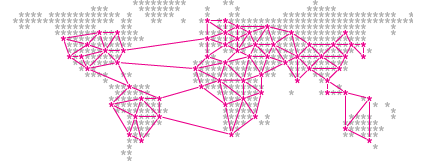
\includegraphics[width=\textwidth]{network-distributed.png}
                \caption{Destributed network [This]}
                \label{fig:Destributed network}
        \end{subfigure}
        \caption{Networks}\label{fig:Networks}
\end{figure}

